\setcounter{part}{28}   % T

\part{Thermodynamique}
\section{Gaz parfaits et réels --- Cinétique des gaz}

% Niveau :      PC
% Discipline :  Thermo
%Mots clés :    Rayonnement du corps noir

\begin{exercise}{Vélo crevé}{2}{Sup}
{Thermodynamique, Gaz parfait, Théorie cinétique des gaz}{bermu,bedo}

On considère une chambre à air d'un pneu de vélo de volume $V$ gonflée à une pression $P_0$. L'air extérieur est sous pression normale atmosphérique $P_\text{a}$ et à température ambiante $T_\text{a}$. Initialement, à $t=0$, la chambre se perce d'un trou de section $s$.

On supposera que la pression $P(t)$ et la température restent uniformes dans le pneu pendant son dégonflement. On supposera également le processus monobare et isotherme.

\begin{questions}
    \questioncours Vitesse quadratique thermique moyenne. On donnera le résultat en fonction des données du problème.
    
    \question Durant $\dd{t}$, estimer le nombre de moles $\dd{n}$ entrant et sortant du pneu par le trou $s$.
    \question En déduire l'équation différentielle régissant la pression du pneu au cours du temps $P(t)$ en fonction de $P_\text{a}$ et d'un temps $\tau$ que l'on introduira et interprétera et la résoudre.
    \question \textsf{Résolution de problème :} lors de la journée nationale de mobilisation contre la réforme des retraites, suite à un mouvement de grève des transports émanant des organisations intersyndicales représentatives de la RATP/SNCF, vous devez vous déplacer à vélo. Mais celui-ci est crevé à cause d'une aiguille de pin. Estimer le temps de dégonflement du pneu de votre vélo.

\end{questions}

\paragraph{Données :}
\begin{itemize}
    \item on modélise l'air comme un gaz parfait diatomique de masse volumique $M = \SI{29}{g\cdot mol^{-1}}$.
    \item constante des gaz parfaits $R = \SI{8,314}{SI}$.
    \item volume d'un tore $V = 2\pi^2 r^2 R$, $r$ est le petit rayon, $R$ le grand rayon.
    \item recommandation de gonflage des pneus de vélo : entre 6 et 8 bar.
\end{itemize}
\end{exercise}

\begin{solution}
\begin{questions}
    \questioncours $\dfrac{5}{2}k_\textsc{b}T = \dfrac{1}{2}mv_q^2\quad$ soit $\quad v_q = \sqrt{\dfrac{5RT}{M}}$.
    \question On modélise la cinétique des gaz comme un mouvement des molécules à $v_q$ dans chacune des 6 directions de l'espace.
    Ainsi, le nombre de particules qui sortent de l'enceinte par $s$ est \\
    $\dd{N}_\text{s} = \dfrac{1}{6}v_q\dd{t} n_\text{int}(t)$ et entrant $\dd{N}_\text{e} = \dfrac{1}{6}v_q\dd{t} n_\text{a}$, $n_\text{int}(t)$ et $n_\text{a}$ étant les densités molaires à l'intérieur et à l'extérieur de l'enceinte.
    \question Donc comme $P(t) = n_\text{int}(t)RT_\text{a}$ et $\dd{P} = RT_\text{a}\dd{N}$, on a 
    $$\dv{P}{t} = - \dfrac{P - P_\text{a}}{\tau}$$
    avec $\tau = \dfrac{6V}{s v_q} = \dfrac{6V}{s}\sqrt{\dfrac{M}{5RT_\text{a}}}$
    \question $P(t) = P_0 + (P_\text{a} - P_0)e^{-t/\tau}$.
    En odg, le diamètre d'un aiguille de pin 2 mm, soit $s \sim \SI{3}{mm^2}$.
    Le volume du pneu : $r = \SI{10}{mm}$, $R=\SI{500}{mm}$, donc $V \sim \SI{1e6}{mm^3}$
    $v_q = $
\end{questions}
\end{solution}

% Niveau :      PCSI
% Discipline :  Thermo
%Mots clés :    Gaz parfaits

\begin{exercise}{Pompe à vélo}{1}{Sup}
{Thermodynamique, Gaz parfait, Théorie cinétique des gaz}{bermu,bedo}

\begin{questions}
    \questioncours Qu'est-ce qu'un gaz parfait ? Donner l'équation d'état du gaz parfait en variables extensives $(V,N)$, intensives $\rho$ (masse volumique) et $n^\ast$ la densité particulaire en $\SI{}{m^{-3}}$.
    
    \question En combien de coup de pompe pour gonfler un pneu de vélo ?
    
    On notera $V_\text{p}$ le volume du piston de la pompe, et $V_\text{c}$ celui de la chambre à air du pneu.

\end{questions}

\paragraph{Données :}
\begin{itemize}
    \item on modélise l'air comme un gaz parfait.
    \item volume d'un tore $V_\text{c} = 2\pi^2 r^2 R$, $r$ est le petit rayon, $R$ le grand rayon.
    \item recommandation de gonflage des pneus de vélo : entre 6 et 8 bar.
\end{itemize}

\end{exercise}

\begin{solution}
\begin{questions}
    \questioncours $pV = nRT$. $pM = \rho R T$. $p = n^\ast k_\textsc{b} T$.
    \question On modélise la situation comme isotherme. Notons $p_n$ la pression dans le pneu de vélo au $n^\text{ème}$ coup de pompe à vélo.

    \textsf{Admission :} on rentre un volume $V_\text{p}$ d'air atmosphérique dans le piston. La quantité de matière correspondante est $n_0 = \dfrac{p_0 V_\text{p}}{R T}$. Elle est toujours la même.

    \textsf{Gonflage :} supposons que la pression dans le pneu est $p_{n-1}$. Lorsqu'on vide les moles du piston dans le pneu, on a une quantité de matière totale est $n_\text{tot} = n_0 + \dfrac{p_{n-1}V_\text{c}}{RT}$. Soit une pression :
    $$p_n = \dfrac{n_\text{tot}RT}{V_\text{c}} = \dfrac{p_0 V_\text{p} + p_{n-1} V_\text{c}}{V_\text{c}}.$$

    \textsf{Conclusion :}

    $$p_n = p_{n-1} + p_0 \dfrac{V_\text{p}}{V_\text{c}} = p_0 \qty(1 + n \dfrac{V_\text{p}}{V_\text{c}}).$$
    donc
    $$n = \dfrac{V_\text{c}}{V_\text{p}}\qty(\dfrac{p_n}{p_0} - 1)$$

    En ODG : $V_\text{c} = 2\pi^2 r^2 R$, $r = \SI{10}{mm}$, $R = \SI {500}{mm}$ soit $V_\text{c} = \SI{1e-3}{m^3}$.
    
    $V_\text{p} =  \pi r^2 h$, $r = \SI{10}{mm}$, $h = \SI{300}{mm}$. $V_\text{p} = \SI{8e-5}{m^3}$.
    
    $\frac{p_n}{p_0} \sim 8$.

    Il faudra donc $n = 60$ coups de pompe.
    
\end{questions}
\end{solution}


% Niveau :      PCSI
% Discipline :  Thermo
%Mots clés :    Gaz parfaits

\begin{exercise}{Atmosphères planétaires}{1}{Sup}
{Thermodynamique, Gaz parfait, Théorie cinétique des gaz}{bermu,perron}

\begin{questions}
    \questioncours Vitesse quadratique thermique moyenne.
    
    \question \`A quelle température l'atmosphère d'une planète s'échappe dans le vide interstellaire ? Quelles planètes du système solaire ne peuvent donc pas avoir d'atmosphère ?

\end{questions}

\paragraph{Données :}~\\[-1ex]
\resizebox{\linewidth}{!}{
\noindent\begin{tabular}{rllllllll}
 & \textbf{Mercure} & \textbf{Venus} & \textbf{Terre} & \textbf{Mars} & \textbf{Jupiter} & \textbf{Saturne} & \textbf{Uranus} & \textbf{Neptune} \\
{ \textbf{Masse $(\SI{1e24}{kg})$}}           & 0.330            & 4.87           & 5.97           & 0.642         & 1898             & 568             & 86.8            & 102              \\
{ \textbf{Rayon ($\SI{}{km}$)}}           & 2440             & 6052         & 6378        & 3396          & 71 492          & 60 268         & 25 559         & 24 764           \\
{ \textbf{Gravité ($\SI{}{m.s^{-2}}$)}}          & 3.7              & 8.9            & 9.8            & 3.7           & 23.1             & 9.0             & 8.7             & 11.0             \\
{\textbf{Vitesse d'échappement ($\SI{}{km/s}$)}}         & 4,3& 10,4& 11,2& 5& 59,5& 35,5& 21,3& 23,5  \\
{ \textbf{Température de surface ($\SI{}{K}$)}}    & 343              & 737            & 288             & 238           & 163           & 133            & 78            & 73             \\
{ \textbf{Composition de l'atmosphère}}    & ??\% O$_2$             & 97\% CO$_2$           & 80\% N$_2$             & 96\% CO$_2$           & 86\% H$_2$          & 96\% H$_2$           & 83\% H$_2$          & 80\% H$_2$            \\
\end{tabular}
}

\noindent\begin{tabular}{lccccc}
 & \textbf{H} & \textbf{He} & \textbf{C} & \textbf{N} & \textbf{O} \\
{ \textbf{Masse molaire $(\SI{}{g.mol^{-1}})$}} & 1 & 2 & 12 & 14 & 16  \\
\end{tabular}

\end{exercise}

\begin{solution}
\begin{questions}
    \questioncours $\dfrac{5}{2}k_\textsc{b}T = \dfrac{1}{2}mv_q^2\quad$ soit $\quad v_q = \sqrt{\dfrac{5RT}{M}}$.
    
    \question Critère : la vitesse de libération est de l'ordre de la vitesse thermique.

\resizebox{\linewidth}{!}{
    \begin{tabular}{rllllllll}
\textbf{Vitesses   thermiques  ($\SI{}{km/s}$)}  & \textbf{Mercure} & \textbf{Venus} & \textbf{Terre} & \textbf{Mars} & \textbf{Jupiter} & \textbf{Saturne} \\
\textbf{N2}                    & 0,63                    & 0,81                     & 0,51                               & 0,43                              & 0,38                                 & 0,34                                 & 0,26                                & 0,26                                 \\
\textbf{O2}                    & 0,59                    & 0,76                     & 0,47                               & 0,40                              & 0,36                                 & 0,32                                 & 0,25                                & 0,24                                 \\
\textbf{CO2}                   & 0,50                    & 0,65                     & 0,40                               & 0,34                              & 0,30                                 & 0,27                                 & 0,21                                & 0,20                                 \\
\textbf{He}                    & 1,17                    & 1,52                     & 0,95                               & 0,81                              & 0,71                                 & 0,64                                 & 0,49                                & 0,48                                 \\
\textbf{H2}                    & 2,34                    & 3,03                     & 1,90                               & 1,61                              & 1,43                                 & 1,29                                 & 0,99                                & 0,96                                 \\
{\textbf{Vitesse d'échappement ($\SI{}{km/s}$)}}         & 4,3& 10,4& 11,2& 5& 59,5& 35,5& 21,3& 23,5
\end{tabular}
}
    
\end{questions}
\end{solution}

\section{Premier principe}
\begin{exercise}{Freinage}{2}{Sup, Spé}
{Thermodynamique,Premier principe,\'Energie interne}{bermudez,bedo}

Une Renault Twingo se déplace à grande vitesse sur une route départementale. Elle freine brusquement et s'arrête.

\begin{questions}
    \questioncours Capacité thermique. Cas des gaz parfaits et des phases condensées.
    \question \textsf{Question ouverte} Estimer l'élévation de température des plaquettes de frein de la voiture suite au freinage. \`A partir de quelle vitesse les freins à disque risquent de ne plus fonctionner correctement ? Est-il pertinent de piler sur les freins passer une certaine vitesse ?
\end{questions}

\paragraph{Données}~(toutes ne sont pas utiles)
\begin{itemize}
    \item Renault Twingo I (2007--2012), 800 kg, $1.4\times1.6\time 3.4$ m, vitesse maximale 170 km/h, 60 ch. max.
    \item Acier inox : densité 8, capacité thermique $\mathrm{500 J\cdot kg^{-1}\cdot K^{-1}}$, point de fusion 1400$^\circ$C
    \item Incandescence des métaux : chauffé au rouge 500$^\circ$C, chauffé à blanc 1200$^\circ$C.  
\end{itemize}

\end{exercise}

\begin{solution}

$\dfrac{1}{2}M v^2 = m c \Delta T$, $M$ étant la masse de la voiture et $m$ celle de la plaquette de freins.

En odg, les plaquettes freins font quelques centimètres et ont une masse d' 1kg environ.

Donc : $\Delta T \ [^\circ\text{C}] = v^2/20 [\mathrm{km/h}]$.

Pour 30 km/h, $\Delta T = 45^\circ$C

On passe au rouge pour 100 km/h, $\Delta T = 500^\circ$C

On passe au blanc pour 150 km/h, $\Delta T = 1200^\circ$C

On passe le point de fusion pour 170 km/h, $\Delta T = 1200^\circ$C

\textsf{Limites :} dissipation de la chaleur par l'air, frottements aérodynamiques de l'air, conduction de la chaleur dans la carrosserie via les essieux.

\end{solution}
\begin{exercise}{Détermination des caractéristiques d'un gaz}{2}{Sup, Spé}
{Thermodynamique}{lelay}

On considère une conduite de section $S$. On place entre son extrémité et un piston une masse $m$ d'un gaz inconnu. On cherche à déterminer les propriétés de ce gaz.

\begin{questions}
    \questioncours Gaz parfaits : équation d'état, énergie interne, capacités thermiques et indice adiabatique (coefficient de Laplace).
    \uplevel{On place dans le conduit de manière transversale un fil de résistance $R$. Initialement, le gaz est à l'équilibre à la température $T_0$}
    \question En partant de la situation d'équilibre et en maintenant le piston en place, on fait passer un courant $I$ dans le fil pendant un temps $\tau$. On constate que la température est passé de $T_0$ à $T_1$. Quelle est l'énergie fournie au gaz ?
    \question On opère la même opération, cette fois-ci en laissant le piston libre de se déplacer. La température passe alors de $T_0$ à $T_2$. S'attend-t-on à avoir $T_1 = T_2$ ?
    \question Déterminer les caractéristiques du gaz.
\end{questions}

\end{exercise}
\begin{exercise}{Boisson fraîche}{2}{Sup, Spé}
{Thermodynamique,Premier principe,Enthalpie,Changement d'état}{bermudez,uhl2019-1}

Lors de la canicule cet été, vous arrivez à cours d'eau fraîche dans votre réfrigérateur. Mais heureusement, il vous reste des glaçons dans votre congélateur et quelques rudiments de thermodynamique... 

\begin{questions}
    \questioncours La fonction d'état enthalpie, $H$. Définition, intérêts et expression du premier principe. On abordera en particulier la question du changement d'état.
    \uplevel{L'idée va être de mélanger les glaçons et l'eau du robinet dans un seau isotherme (de champagne par exemple) pour obtenir de l'eau fraîche.}
    \question \textsf{Question ouverte} Combien faut-il de glaçons $N_\text{g}$ et d'eau du robinet $V_\ell$ (en mL) pour obtenir à la fin 1L ($M = 1$ kg) d'eau fraîche ? \\
    On notera $T_\text{a}$ la température ambiante, $T_\text{g}$ la température de la glace, $T_\text{f}$ la température du frigidaire. \\
    \textsl{Le raisonnement se basera sur des estimations d'ordres de grandeur et sur les données ci-après.}
\end{questions}

\paragraph{Données}~(toutes ne sont pas utiles)
\begin{itemize}
    \item masse volumique de la glace $\rho_\text{g} = 920 \ \mathrm{kg\cdot m^{-3}}$ ;
    \item masse d'un galçon $m_\text{g}$ : à estimer ;
    \item enthalpie massique de fusion de l'eau à $0^\circ$ C, $\Delta_\text{fus}\cal{h} = 330\ \mathrm{kJ\cdot kg^{-1}}$ ;
    \item enthalpie massique de vaporisation de l'eau à 100$^\circ$ C, $\Delta_\text{vap}\cal{h} = 2300\ \mathrm{kJ\cdot kg^{-1}}$ ;
    \item capacité thermique massique de l'eau à 300 K, $\cal{c}_\ell$ : définition de la calorie ;
    \item capacité thermique massique de la glace à $0^\circ$ C, $\cal{c}_\text{g} =  2.1\ \mathrm{kJ\cdot kg^{-1}\cdot K^{-1}}$ ;
    \item capacité thermique massique de l'inox à 300 K, $\cal{c}_\text{i} =  0.5\ \mathrm{kJ\cdot kg^{-1}\cdot K^{-1}}$ ;
    \item masse du seau à champagne $m_\text{i} = 500$ g.
    
\end{itemize}

\end{exercise}

\begin{solution}
Le système $\scr{S}$ : $\{$ glace $+$ eau $+$ seau $\}$. On a par hypothèse $\Delta H(\scr{S}) = 0$ ainsi que la conservation de la masse $N_\text{g} m_\text{g} + \rho_\ell V_\ell = M = 1$ kg.

ODG non fournis :
\begin{itemize}
    \item $\cal{c}_\ell = 4.18\ \mathrm{kJ\cdot kg^{-1}}$
    \item $T_\text{f} = 4^\circ$C, $T_\text{g} = -18^\circ$C, $T_\text{a} = 30^\circ$ C.
    \item $m_\text{g} = 10$ g
\end{itemize}

Étapes de la réaction :
\begin{itemize}
    \item les glaçons se réchauffent à $T_\text{fus}$ ;
    \item les glaçons fondent ;
    \item l'eau de glaçon fondue se réchauffe à $T_\text{f}$ ;
    \item l'inox et l'eau se refroidissent à $T_\text{f}$ ;
\end{itemize}
soit
$$N_\text{g} m_\text{g} \cal{c}_\text{g} (T_\text{fus} - T_\text{g}) + N_\text{g} m_\text{g}\Delta_\text{fus}\cal{h} + N_\text{g} m_\text{g} \cal{c}_e (T_\text{f} - T_\text{fus}) + (\rho_\ell V_\ell \cal{c}_\ell + m_\text{i} \cal{c}_\text{i})(T_\text{f} - T_\text{a}) = 0.$$
En substituant $V_\ell$ par $(M - N_\text{g} m_\text{g})/\rho_\ell$, on trouve

$$N_\text{g} = -\dfrac{1}{m_\text{g}}\dfrac{(M \cal{c}_\ell + m_\text{i} \cal{c}_\text{i})(T_\text{a} - T_\text{f})}{\cal{c}_\text{g}(T_\text{fus} - T_\text{g}) + \Delta_\text{fus}\cal{h} + \cal{c}_\ell(T_\text{a} - T_\text{fus})} \sim 10 \text{ glaçons}$$

$$V_\ell = 925\text{ mL}$$

\end{solution}
\begin{exercise}{Extinction massive du Crétacé--Paléogène}{2}{Sup, Spé}
{Thermodynamique,Premier principe,Enthalpie,Changement d'état}{bermudez,bedo}

Il y a 66 millions d'année, une comète de 5 km de rayon s'est écrasée sur Terre, formant l'actuel Golfe du Mexique et causant une extinction massive qui a fait disparaître environ 50\% des espèces présentes sur Terres, notamment les dinosaures.

\begin{questions}
    \questioncours Gaz parfait. Hypothèses. Expressions des lois de Joule et de Laplace.
    \uplevel{Lorsqu'elle s'est écrasée, la comète à provoqué un réchauffement planétaire global.}
    \question Interpréter cette affirmation d'un point de vue énergétique.
    \question Par conservation de l'énergie mécanique avant l'impact, évaluer la vitesse et l'énergie cinétique de la comète avant l'impact. On notera $M$ la masse de la comète.
    \uplevel{On peut estimer qu'une part de cette énergie a vaporisé l'océan qui se trouvait sur le lieu de l'impact.}
    \question \'Evaluer cette énergie. Conclure quant aux ordres de grandeurs de cette énergie et de celle initiale de la comète.
    \uplevel{Il est estimé que les roches de la comète ont été instantanément liquéfiées vaporisées et que l'énergie restante à été convertie sous forme de rayonnement thermique.}
    \question \'Evaluer ces énergies.
    \question Tout le rayonnement a-t-il pu être converti sous forme de transfert thermique pour réchauffer l'atmosphère ?
    \question Estimer enfin l'élévation en température atmosphérique causée par ce cataclysme.
    \question Commenter le résultat. Quelles autres causes pourraient avoir contribué au réchauffement global suite à l'impact de la comète ?
\end{questions}

\paragraph{Données}~(toutes ne sont pas utiles)
\begin{itemize}
    \item la comète est constituée principalement de roches et d'iridium de densité 3 ;
    \item enthalpie massique de vaporisation de l'eau à 100$^\circ$ C, $\Delta_\text{vap}\cal{h} = 2300\ \mathrm{kJ\cdot kg^{-1}}$ ;
    \item enthalpie massique de liquéfaction des roches à 1500 K, $\Delta_\text{fus}\cal{h} ~ 10^3\ \mathrm{kJ\cdot kg^{-1}}$ ;
    \item enthalpie massique de liquéfaction des roches à 3000 K, $\Delta_\text{fus}\cal{h} ~ 10^4\ \mathrm{kJ\cdot kg^{-1}}$ ;
    \item capacité thermique massique de l'eau à 300 K : définition de la calorie ;
    \item capacité thermique massique des roches à 300 K, $\cal{c} = 300\ \mathrm{J\cdot kg^{-1}\cdot K^{-1}}$ ;
    \item rayon de la terre $R_\textsc{t} = 6400$ km ;
    \item accélération normale de la pesanteur terrestre $g$ : à connaître ;
    \item indice adiabatique de l'air $\gamma = 1.4$ ;
    \item constante des gaz parfaits $R$ : à connaître ;
    \item pression atmosphérique $P_0$ : à connaître ;
\end{itemize}

\end{exercise}

\begin{solution}
Le système $\scr{S}$ : $\{$ glace $+$ eau $+$ seau $\}$. On a par hypothèse $\Delta H(\scr{S}) = 0$ ainsi que la conservation de la masse $N_\text{g} m_\text{g} + \rho_\ell V_\ell = M = 1$ kg.

\begin{questions}
    \questioncours
    \question Energie cinétique => énergie utile à chauffer l'atmosphère + pertes
    \question $E_\text{pp}(r) = -\dfrac{G M M_\textsc{t}}{r} = -M g \dfrac{R_\textsc{t}^2}{r}$. D'où $E_\text{c,f} = M g R_\textsc{t} = 10^{23}$ J.
    \question Si on suppose une vaporisation de la taille de la comète environ $E = 10^{19}$ J : négligeable
    \question Cette fois-ci avec les ODG des roches on trouve plus normalement
    \question La moitié du rayonnement est convertie : 1/2 du rayonnement par vers le haut (atmosphère), 1/2 vers le bas. Donc $Q \sim 10^{23}$ J
    \question On a donc $\Delta U = Q = m c\Delta T$. $c = \dfrac{R}{\gamma - 1}$.
    Masse de l'atmosphère à estimer avec $P_0$. On trouve $\Delta T = 42$ K !
    \question Effet de serre...
\end{questions}

\end{solution}
\begin{exercise}{Système thermomécanique}{2}{Sup, spé}
{Thermodynamique}{lelay}

On considère un système thermomécanique définit comme suit : Dans un conduit vide de section $S$ et de longueur $\ell_0$, on place une paroi reliée à une extrémité du conduit par un ressort de raideur $k$ et de longueur à vide $\ell_0$. Entre l'autre extrémité et la paroi, on place une certaine quantité d'un gaz du indice adiabatique $\gamma$.

\begin{center}
    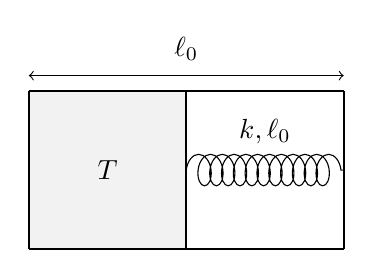
\begin{tikzpicture}
    \draw[<->] (0,1.2) -- (4, 1.2);
    \draw (2,1.2) node[above=2pt] {$\ell_0$};
    
    \fill[black!5]  (0,-1) rectangle (2,1);
    \draw[thick] (0,-1) -- (0, 1);
    \draw[thick] (0,-1) -- (4,-1);
    \draw[thick] (0, 1) -- (4, 1);
    \draw[thick] (2,-1) -- (2, 1);
    \draw (1,0) node[anchor=center] {$T$};
    
    \draw[decoration={aspect=0.6, segment length=1.5mm, amplitude=2mm,coil},decorate] (2,0) -- (4,0);
    \draw[thick] (4,-1) -- (4, 1);
    \draw (3,0) node[above=6pt] {$k, \ell_0$};
    
    \end{tikzpicture}
\end{center}

\begin{questions}
    \questioncours Capacités thermiques et coefficient isentropique.
    \question Initialement, le gaz est à la température $T$. Exprimer l'énergie potentielle du ressort en fonction de $T$.
    \question On fournit une certaine quantité de chaleur $Q$ au système. Que se passe-t-il ? 
    \question Donner la définition et exprimer ${C_{V}}_{m}$ la capacité thermique isochore molaire du système étudié.
\end{questions}

\end{exercise}

\begin{solution}

\begin{questions}
    \questioncours $c_p = c_v + nR$
    \question Si on note $x$ le déplacement du ressortr, alors $V = x S$, $P = kx/S$ hence $E_p = \frac12 kx^2 =\frac12 PV$. Or $PV =nRT$ d'où $E_p = nRT/2$
    \question Ca bouge. Bilan d'énergie : $Q = \Delta U_\text{gaz} + \Delta E_p = c_v \Delta T + nR/2\Delta T$
    \question  ${C_{V}}_{m} = \Delta U_\text{tot}/\Delta T = c_v + nR/2$
\end{questions}

\end{solution}

\section{Second principe}
\begin{exercise}{Bilan entropique}{2}{Sup, Spé}
{Thermodynamique}{lelay, X}

On considère un récipient calorifugé de volume $V_0$ et de section $\Sigma$. Dans ce récipient est placé une paroi mobile.

\begin{questions}
    \questioncours Principes de la thermodynamique.
    \uplevel{On place dans la partie gauche du récipient $n$ moles d'un gaz diatomique à la température $T_1 = T_0$ et dans la partie droite $n$ moles de ce même gaz à la température $T_2 = 3T_0$. On relâche la paroi.}
    \question Rappeler la différence entre équilibre mécanique et équilibre thermodynamique. Lequel est le plus rapide à s'établir ?
    \question Peu de temps après avoir relâché la paroi, quels sont les volumes $V_1$ et $V_2$ occupées par gaz à gauche et à droite de la paroi ? Les pressions $P_1$ et $P_2$ ?
    \question Même question après avoir attendu un temps long.
    \question Faire un bilan entropique pour chacun des gaz. Quelle est l'entropie totale créée par cette opération ?
\end{questions}

\end{exercise}

\begin{solution}

\begin{questions}
    \questioncours 0 1 2 3 4
    \uplevel{On place dans la partie gauche du récipient $n$ moles d'un gaz diatomique à la température $T_1 = T_0$ et dans la partie droite $n$ moles de ce même gaz à la température $T_2 = 3T_0$. On relâche la paroi.}
    \question Équilibre méca plus rapide, sauf chelouterie
    \question Les températures sont tj $T_1$ et $T_2$, à l'équilibre méca les pressions s'égalisent : $P = nRT_1/V_1 = nRT_2/V_2$ d'où $V_1 = V_0/4$ et $V_2 = 3V_0/4$
    \question Ce coup ci les températures se sont équilibrées, $T_1=T_2 = 2T_0$, $V = V_0/2$ et $T = 2T_0$
    \question $\dd{U}= C_v \dd{T} = T\dd{S} -P\dd{V}$ hence $\dd{S} = C_v \dd{T}/T + nR\dd{V}/V$. 

    À gauche : $\Delta S_1 = C_v \ln(2T_0/T_0) + nR\ln(\frac{V_0/2}{V_0/4}) = (C_v+nR)\ln(2)$

    À droite : $\Delta S_2 = C_v \ln(2T_0/3T_0) + nR\ln(\frac{V_0/2}{3V_0/4}) = (C_v+nR)\ln(2/3)$

    En tout $\Delta S = \Delta S_1 + \Delta S_2 = (C_v + nR)(\ln(2)+\ln(2/3)) = C_p \ln(4/3)$
\end{questions}

\end{solution}

\begin{exercise}{Transition de phase --- Idées reçues}{0}{Sup, Spé}
{Thermodynamique,Changement d'état}{bermudez}

\begin{questions}
    \questioncours Corrigez les affirmations ci-dessous
    \begin{parts}
        \part Un changement d'état à lieu à température et pression constantes.
        \part Au cours d'un changement d'état isotherme d'un corps pur, l'énergie interne ne varie pas.
        \part Au cours de la vaporisation isotherme d'un corps pur, la variation d'énergie interne est égale à la chaleur latente de vaporisation.
        \part Au point triple, l'état du système est parfaitement déterminé.
    \end{parts}
\end{questions}

\end{exercise}

\begin{solution}

\begin{questions}
    \questioncours ~
    \begin{parts}
        \part La variance est de 2, donc \emph{imposer la pression et la quantité de matière du système revient à imposer également la température} : la relation $P(T,n)$ est fixée, mais pas $(P,T,n)$ individuellement.
        \part Elle varie
        \part C'est la variation d'enthalpie qui est égale à la chaleur latente.
        \part Au point triple, la variance est de 1, donc $P(n),T(n)$ sont fixés \emph{seulement si $n$ est fixé, i.e.} si le système est fermé.
    \end{parts}
\end{questions}

\end{solution}

\section{Machines thermiques}
\begin{exercise}{Rendement de Curzon et Alhborn}{4}{Sup, spé}
{Thermodynamique, Machine thermique}{lelay,CurzonAhlborn1975}

\begin{questions}
    \questioncours Rappeler la forme du cycle de Carnot et démontrer la formule de l'efficacité de Carnot : $\eta = 1 -\frac{T_f}{T_c}$
    \question Est-il possible d'obtenir le rendement de Carnot avec une machine thermique réelle ? Que faut-il faire pour s'en approcher ? Quel problème pratique cela pose-t-il, au niveau de la puissance par exemple ?
\uplevel{En vue d'applications dans la vie réelle, on souhaite maintenant optimiser non pas l'efficacité mais la puissance de notre machine thermique.}    
    \question On considère un moteur de Carnot modifié tel que 
    \begin{enumerate}
        \item La détente isotherme à haute température se produit à température $T_1$ pendant un temps $t_1$, durant cette phase le moteur reste en contact avec le réservoir chaud à température $T_c > T_1$.
        \item La compression isotherme à basse température se produit à température $T_2$ pendant un temps $t_2$, durant cette phase le moteur reste en contact avec le réservoir foid à température $T_f < T_2$.
        \item Les phases adiabatiques sont très rapides, leur durée est négligeable.
    \end{enumerate}
    En utilisant le premier principe, calculer la puissance $W$ de ce moteur en fonction de $T_1$, $T_c$, $T_2$, $T_f$, $t_1$, $t_2$ et $C$.
    \question On pose $x = 1 - T_1/T_c$ et $y = T_2/T_f-1$. Quel est le signe de $x$ et de $y$ ? En utilisant le second principe, exprimer $\frac{t_1}{t_2}$ en fonction de $x$, $y$, $T_c$ et $T_f$.
    \question En remplaçant $\frac{t_1}{t_2}$ dans l'expression de la puissance, exprimer la puissance réduite $P' = P/C$ en fonction de $x$, $y$, $T_c$ et $T_f$.
    \question On cherche à maximiser la puissance de notre machine thermique. Comment exprimer cela mathématiquement ? 
    \question En se plaçant au point de puissance optimale, montrer que le rapport $\frac{y}{x}$ revêt une forme simple.
    \question Le rendement de cette machine thermique est $\eta' = 1-\frac{y}{x}\frac{T_f}{T_c}$. Discuter du rapport avec le rendement de Carnot.
    \question La table ci dessous est tirée de l'article original de Curzon et Ahlborn (1975). Calculer pour chaque centrale le rendement de Carnot et le rendement $\eta'$ de Curzon et Alhborn. Commenter.
\end{questions}

\begin{figure}[H]
    \centering
    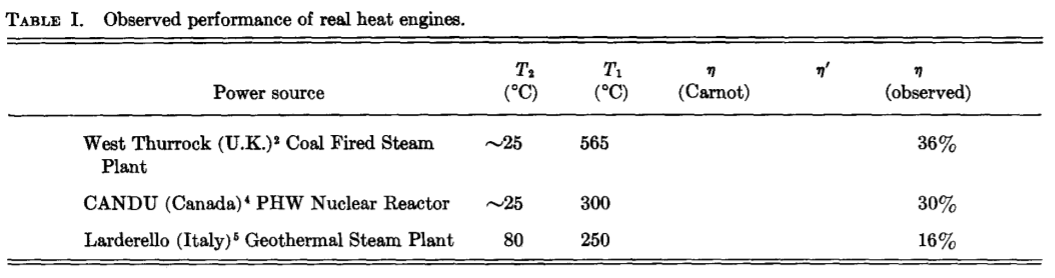
\includegraphics[width=0.9\textwidth]{thermo/machinesthermiques/RendementsCA.png}
    \caption{Table de rendements.}
\end{figure}

\end{exercise}

\begin{solution}
\begin{questions}
    \questioncours $\eta = 1 -\frac{T_f}{T_c}$
    \question Non, il faut attendre un temps infini : puissance nulle.
\uplevel{En vue d'applications dans la vie réelle, on souhaite maintenant optimiser non pas l'efficacité mais la puissance de notre machine thermique.}    
    \question Il faut traduire les données de l'énoncé
    \begin{enumerate}
        \item $Q_1 = C(T_c-T_1) t_1$.
        \item $Q_2 = C(T_2-T_f) t_2$.
        \item On reste sur un semi - moteur de Carnot, donc $\Delta S_{c} = 0$
    \end{enumerate}
    Le premier principe donne $W - Q_1 + Q_2 = 0$ et $P = \frac{W}{t_1+t_2}$, d'où
    \begin{align*}
        P = \frac{Q_1 - Q_2}{t_1+t_2} = \frac{C(T_c-T_1) t_1 - C(T_2-T_f) t_2}{t_1+t_2}
    \end{align*}
    L'EXO EST FAISABLE AVEC $C_1 \neq C_2$ IL EST JUSTE PLUS CHAUD.
    \question $x > 0$, $y > 0$, Le second principe donne $Q_1/T_1 = Q_2/T_2$ d'où 
    \begin{align*}
        \frac{t_1}{t_2} &= \frac{y}{x}\frac{1-x}{1+y}
    \end{align*}
    \question $P' = \frac{ xy\qty( (1-x)T_c ) - (1+y)T_f }{ x(1+y) + y(1-x) }$
    \question On veut $\pdv{P}{T_1} = \pdv{P}{T_2} = 0$ hence $\pdv{P'}{x} = \pdv{P'}{y} = 0$
    \question Les calculs sont violents, on trouve $\frac{y}{x} = \sqrt{\frac{T_c}{T_f}}$
    \question Pouit pouit la racine
\end{questions}
\end{solution}
\begin{exercise}{Maison au bord du lac}{3}{Sup, spé}
{Thermodynamique,machines thermiques,pompe à chaleur}{lelay}

On considère un bûcheron (fin)landais habitant une maison au bord d'un lac près la mer du Nord. L'eau du lac est à 5 degrés Celsius, l'air ambiant est à $-10$ degrés Celsius. Le but de cet exercice est de déterminer si le bûcheron arrivera à chauffer sa maison à 20 degrés (sans utiliser de bois !).

\begin{questions}
    \questioncours Principes thermodynamiques appliqués aux machines thermqiues, rendement de Carnot.
    \question Faire un schéma, incluant des petits poissons dans le lac, des oiseaux dans le ciel et un chat dans la maison du bûcheron.
    \question Le bûcheron souhaite chauffer sa maison. Peut-il y arriver sans utiliser le lac ?
    \question Montrer que le bûcheron peut se servir d'une machine thermique pour générer du travail. Comment alors utiliser ce travail pour chauffer sa maison ? Quelle est l'entropie créée par ce procédé ?
    \question Le bûcheron (qui est un peu excentrique) souhaite en fait se chauffer de manière isentropique. Comment faire ?
    \question Définir et calculer l'efficacité de ce procédé selon la méthode utilisée.
    \question Retrouver le résultat grâce à une méthode plus simple
\end{questions}

\end{exercise}

\begin{solution}
\begin{questions}
    \questioncours Principes thermodynamiques appliqués aux machines thermiques, rendement de Carnot.
    \question 
\begin{center}
    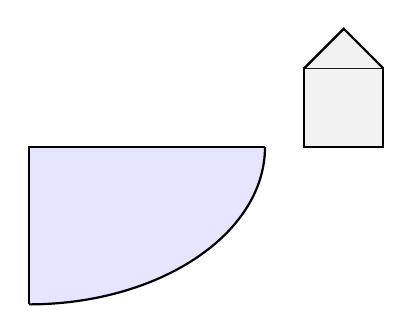
\begin{tikzpicture}
    \tikzset{
    partial ellipse/.style args={#1:#2:#3}{
        insert path={+ (#1:#3) arc (#1:#2:#3)}
    }
    }
    \fill[fill=blue!10] (0,0) -- (0,-2) -- (3,0);
    \filldraw[thick, color=black, fill=blue!10] (0,0) [partial ellipse=-90:0:3 and 2];
    \draw[black, thick] (0,-2) -- (0,0) -- (3,0);
    
    \filldraw[color=black, thick, fill=black!5] (3.5,0) rectangle (4.5,1);
    \filldraw[color=black, thick, fill=black!5] (3.5,1) -- (4,1.5) -- (4.5,1);
    
    \end{tikzpicture}
\end{center}
    \question Non, à cause du second principe.
    \question Il fait une machine thermique entre le lac et l'air, générant un travail $W$. Il peut convertir ce travail par exemple avec ue résistance chauffante. L'entropie produite est alors $W/T$ avec $T$ la température de la maison.
    \question Il branche la machine thermique de la question précédente sur une autre machine thermique chauffante isentropique. La source chaude est alors la maison et la source froide est soit l'air (moins efficace car plus froid, mais permet d'utiliser de l'énergie pas chère puisqu'on s'en fout de le refroidir) soit le lac (plus efficace, mais on refroidit plus le lac). 
    \question L'air on s'en fiche, on veut optimiser $Q$ le transfert thermique à la maison par rapport à $Q_\ell$ le transfert thermique au lac (pour ne pas le faire geler). On trouve 
    \begin{align*}
        \frac{Q}{Q_\ell} &= \frac{T_\ell - T_a}{T - T_\ell}\frac{T}{T_\ell}
    \end{align*}
    \question Utiliser une machine tritherme ne générant pas de travail.
\end{questions}
\end{solution}
\begin{exercise}{Machine thermique non stationnaire}{2}{Sup, spé}
{Thermodynamique}{lelay}

On considère un moteur ditherme $M$, en contact avec deux réservoirs à la température $T_1$ et $T_2$ avec $T_1 > T_2$.

\begin{questions}
    \questioncours Qu'est ce qu'une machine thermique ?
    \question Dans le cas présent quelle est la source chaude ? Froide ? Faire un schéma en précisant le sens des échanges.
    \question On considère maintenant que les réservoirs sont \emph{finis}. Qu'est-ce que cela implique ? 
    \uplevel{Les températures initiales des réservoirs sont notées $T_{10}$ et $T_{20}$. On considère que le temps de variations de température des réservoirs est grand devant le temps d'un cycle de la machine. On suppose que les réservoirs sont de même nature et ont une capacité thermique $c$.}
    \question Le moteur peut-elle fonctionner un temps infini ? Pourquoi ?
    \question Exprimer le travail total fourni par le moteur en fonction de $c$, $T_{10}$, $T_{20}$ et $T_f$.
    \question Montrez que, dans le cas isentropique, on a l'identité $T_1T_2 = K$ avec $K$ une constante. Quel est alors le travail total fourni ?
    \question Montrez que cette situation est la plus favorable.
\end{questions}

\end{exercise}

\begin{solution}
\begin{questions}
    \questioncours Qu'est ce qu'une machine thermique ?
    \question $T_1$ chaude, $T_2$ froide, $Q_1 > 0$, $Q_2 < 0$. Et évidemment $W < 0$ (moteur).
    \question Capacité thermique $\neq \infty$ : la source froide va se réchauffer et la source chaude se refroidir
    \uplevel{Les températures initiales des réservoirs sont notées $T_{10}$ et $T_{20}$. On considère que le temps de variations de température des réservoirs est grand devant le temps d'un cycle de la machine. On suppose que les réservoirs sont de même nature et ont une capacité thermique $c$.}
    \question Non, $T_1$ décroît, $T_2$ croît et à la fin on aura $T_1 = T_2 = T_\text{f}$ und es gibt keine moteur monotherme.
    \question D'après l'approximation, on a toujours $W = -Q_1-Q_2$ et donc $W_\text{tot} = \sum W = -\sum Q_1 - \sum Q_2$. Or d'après le premier principe appliqué à chaque réservoir, $Q_1 = -c\dd{T_1}$ et $Q_2 = -c\dd{T_2}$ d'où $W_\text{tot} = c\qty(\int \dd{T_1} + \int\dd{T_2}) = c(2T_\text{f} - T_{10} - T_{20})$
    
    Remarque : Dans le "meilleur" des cas on extrait un max de travail (en valeur absolue) quand $W$ est minimum, i.e. $T_\text{f} = T_{20}$, et alors $\abs{W_\text{tot}^\text{max}} = c(T_{10}-T_{20})$. Bien sûr c'est impossible, ça voudrait dire que la source froide ne se réchauffe pas alors que la source chaude se refroidit, i.e. $Q_2  =0$, c'est en fait un moteur monotherme déguisé ! Au contraire, dans le "pire" des cas on a $W_\text{tot} = 0$ i.e. $T_\text{f} = (T_{10}+T_{20})/2$ ce qui correspond à la situation où les deux réservoirs sont en contact thermique simple (et évidemment dans cette situation aucun travail n'est fourni). On a donc $T_\text{f}$ qui est plus proche de $T_{20}$ que de $T_{10}$ : nécessairement la source chaude se refroidit plus vite que la source froide ne se réchauffe.
    \question Dans le cas isentropique, on écrit $\Delta S = -Q_1/T_1-Q_2/T_2 = 0$ (sur un cycle). On a alors $\dd{T_1}/T_1 + \dd{T_2}/T_2 = 0$ et donc $T_1T_2 = K$. On en déduit $T_\text{f} = \sqrt{T_{10}T_{20}}$. La moyenne géométrique étant toujours plus petite que la moyenne arithmétique, ça marche. On en déduit $\abs{W_\text{tot}} = \sqrt{T_{10}} - \sqrt{T_{20}}$
    \question Si $S_\text{cree}$ sur un cycle est positive, alors $\dd{T_1}/T_1 + \dd{T_2}/T_2 > 0$, $T_1T_2$ croît et $T_\text{f} > \sqrt{T_{10}T_{20}}$.
\end{questions}
\end{solution}
\begin{exercise}{Machine thermique semi-stationnaire}{2}{Sup, spé}
{Thermodynamique}{lelay}

On considère un moteur ditherme $M$, en contact avec deux réservoirs : l'un est l'air ambiant à la température $T_a$, l'autre est un matériau chaud, à la température $T_c > T_a$, possédant une capacité thermique $c$.

\begin{questions}
    \questioncours Qu'est ce qu'une machine thermique ?
    \question On considère ce moteur isentropique. Quelle est la puissance qu'il génère dans l'approximation $c \longrightarrow \infty$ ? La reconnaissez vous ?
    \question Que va-t-il se passer si $c \neq \infty$ ? Vers quoi tendra $T_c$ la température de la source chaude ? En déduire le travail maximum théorique que l'on peut songer à extraire de ce moteur.
    \uplevel{Les température initiale de la source chaude est notée $T_0$. On considère que le temps typique de variations de $T_c$ est grand devant le temps d'un cycle de la machine.}
    \question On suppose d'abord que la puissance fournie par la source chaude $P_c$ est constante.
    \begin{parts}
        \part Donner l'expression de $T_c(t)$ et représenter graphiquement cette fonction. À partir de quel instant $t_{max}$ le moteur cessera-t-il de fonctionner ?
        \part Exprimer $P(t)$ la puissance mécanique fournie par le moteur en fonction du temps. Que vaut $P(t=0)$ ? $P(t=t_{max})$ ? $P(t > t_{max})$ ?
        \part Montrez que le travail total fourni par le moteur est
        \begin{align*}
            W &= c(T_0 - T_a) - cT_a \ln{\frac{T_0}{T_a}}
        \end{align*}
    \end{parts}
    \question Cette fois, on cherche à ce que le moteur fournisse une puissance mécanique $P$ constante.
    \begin{parts}
        \part Quel est l'intérêt pratique de cette situation ?
        \part Montrez que la quantité $x = \frac{T_c}{T_f}$ obéit à l'équation
        \begin{align*}
            \tau \dv{x}{t}  = \frac{x}{1-x}
        \end{align*}
        On précisera l'expression de $\tau$ et sa dimension.
        \part En faisant une approximation que l'on justifiera, montrer que l'on peut écrire $T_c = T_0 - \frac{Pt}{c}$. À partir de quand le moteur cessera-t-il de fournir du travail ?
        \part Montrez que le travail total fourni par le moteur est
        \begin{align*}
            W &= c(T_0 - T_a)
        \end{align*}
    \end{parts}
\end{questions}

\end{exercise}

\begin{solution}
\begin{questions}
    \questioncours Qu'est ce qu'une machine thermique ?
    \question Carnot $1 - T_c/T_f$
    \question $T_c \longrightarrow T_f$, max is $c(T_c(0)-T_f)$
    \uplevel{Les température initiale de la source chaude est notée $T_0$. On considère que le temps typique de variations de $T_c$ est grand devant le temps d'un cycle de la machine.}
    \question On suppose d'abord que la puissance fournie par la source chaude $P_c$ est constante.
    \begin{parts}
        \part $T_c = T_0 - P_ct/c$, le moteur s'arrête lorsque $T_c=T_c$ i.e. $t = (T_0-T_f)c/P_c$
        \part $P = P_c - P_f$, avec le second principe on a $P_f = f(P_c)$. 
        \part Il faut juste intégrer
    \end{parts}
    \question Cette fois, on cherche à ce que le moteur fournisse une puissance mécanique $P$ constante.
    \begin{parts}
        \part On a tout le temps le meme travail c pratik
        \part C'est la condition isentropique, $\tau = c T_f / P$
        \part On résoud par séparation des variables et on trouve $\dd{\qty(x(1-\ln{x}/x))} = -\dd{t}/\tau$, on suppose que $\ln(x)/x \ll 1$ (c'est vrai en $1$, en $\infty$, et le max c'est $1/e$ donc ça passe), tout s'arrête à $\tau(\frac{T_0}{T_f}-1)$
        \part Pareil il faut juste intégrer. On tombe sur l'optimum (merci l'approximation).
    \end{parts}
\end{questions}
\end{solution}

\section{Systèmes ouverts}
\begin{exercise}{Centrale nucléaire du Blayais  }{2}{Sup, spé}
{Thermodynamique, Machines thermiques, Premier principe industriel}{bermudez,uhl2019-1}

La centrale nucléaire du Blayais, suitée dans l'estuaire de la Gironde, à 50 km en aval de Bordeaux, est constituée de 4 réacteurs à eau pressurisée (REP --- 70 bars, 350$^\circ$ C), refroidis par l'eau de l'estuaire qui est pompée via des canalisations sous-marines.

\textsf{Question ouverte : } \`A l'aide des données suivantes :
\begin{questions}
    \question Estimez le rendement de la centrale nucléaire. Commenter.
    \question Comparez ce rendement avec celui de Carnot ainsi que le rendrement à puissance maximale $\eta_\text{pmax} = 1 - \sqrt{T_\text{f}/T_\text{c}}$.
    \question Estimez l'échauffement de l'eau de l'estuaire en aval de la centrale. La législation impose un échauffement maximal de $+3^\circ$ C ; est-elle respectée ?
\end{questions}

% Please add the following required packages to your document preamble:
% \usepackage{multirow}
\begin{table}[H]
\begin{tabularx}{\linewidth}{llCCCrrr}
\multicolumn{1}{c}{\multirow{2}{*}{\textsfbf{\begin{tabular}[c]{@{}c@{}}Nom du\\ réacteur\end{tabular}}}} & \multicolumn{1}{c}{\multirow{2}{*}{\textsfbf{Modèle}}} & \multicolumn{3}{c}{\textsfbf{Capacité {[}MW{]}}}                                                                                      & \multicolumn{1}{c}{\multirow{2}{*}{\textsfbf{\begin{tabular}[c]{@{}c@{}}Début\\ constr.\end{tabular}}}} & \multicolumn{1}{c}{\multirow{2}{*}{\textsfbf{\begin{tabular}[c]{@{}c@{}}Raccord\\ au réseau\end{tabular}}}} & \multicolumn{1}{c}{\multirow{2}{*}{\textsfbf{\begin{tabular}[c]{@{}c@{}}Mise en\\ service\end{tabular}}}} \\
\multicolumn{1}{c}{}                                                                                    & \multicolumn{1}{c}{}                                 & \textsfbf{thermique} &\textsfbf{brute} & \textsfbf{nette} & \multicolumn{1}{c}{}                                                                                  & \multicolumn{1}{c}{}                                                                                      & \multicolumn{1}{c}{}                                                                                            \\ \hline
Blayais-1                                                                                            & CP1                                                  & 2 785                                         & 951                                      & 910                                      & janvier 1977                                                                                          & juin 1981                                                                                                 & déc. 1981                                                                                                   \\
Blayais-2                                                                                              & CP1                                                  & 2 785                                         & 951                                      & 910                                      & janvier 1977                                                                                          & juillet 1982                                                                                              & fév. 1983                                                                                                    \\
Blayais-3                                                                                              & CP1                                                  & 2 785                                         & 951                                      & 910                                      & avril 1978                                                                                            & août 1983                                                                                                 & nov. 1983                                                                                                   \\
Blayais-4                                                                                              & CP1                                                  & 2 785                                         & 951                                      & 910                                      & avril 1978                                                                                            & mai 1983                                                                                                  & oct. 1983                                                                                                      
\end{tabularx}
\end{table}

\paragraph{Données :} débit moyen annuel de la Gironde à Blayes $\SI{950}{}$ m$^3\cdot$s$^{-1}$.

\end{exercise}

\begin{solution}

    \begin{questions}
        \question $\eta = \dfrac{\text{P brute}}{\text{P thermique}} = 35\%$
        \question Si on prend $T_f = 25^\circ$ C, l'eau de la Gironde en hiver, et $T_c = 350^\circ$ soit un rendement de Carnot de 52\% et de Curzon de 35\%
        \question La puissance envoyée dans l'eau est environ $P_f = 4\times (2785 - 951) = 7,4$ GW. On a donc
        $$\delta Q = \dd{m} c_m \Delta T \qqtext{soit} \Delta T = \dfrac{P_f}{D_v \rho c_m}$$

        AN :         $\Delta T = 1,8^\circ$ C.

        On peut donner $c = 4,18$ J/g/K si il y a un trou de mémoire
    \end{questions}
\end{solution}
\begin{exercise}{Refroidisseur à eau}{1}{Sup, spé}
{Thermodynamique, Premier principe industriel}{lelay,centrale}

\begin{questions}
    \questioncours Principes de la thermodynamique en régime ouvert
    \uplevel{On considère un refroidisseur à eau, un système dans lequel circule de l'air et de l'eau. L'air entre dans le dispositif à la température $T_1 = 500$ K et en sort à la température $T_2 = 300$ K avec un débit de sortie de 65 L/s. En entrée et en sortie l'air est à pression atmosphérique. L'eau rentre à la température $\Theta_e = 12$ degrés Celsius avec un débit de 1 L/s et sort à la température $\Theta_s$.}
    \question Calculer $\Theta_s$.
\end{questions}

\end{exercise}

\begin{solution}
C'est juste le premier principe industriel. Il faut savoir retrouver la masse molaire de l'air (29 g/mol).
\end{solution}
\begin{exercise}{Tuyère de De Laval}{3}{Sup, spé}
{Thermodynamique, Premier principe industriel}{lelay,centrale}

\begin{questions}
    \questioncours Premier principe de la thermodynamique en régime ouvert
    \uplevel{On considère une tuyère (ex : réacteur d'avion, de fusée) dans laquelle le fluide se déplace de manière unidimensionnelle avec une vitesse $V(x)$.}
    \question Écrire le premier principe industriel et montrer qu'entre deux abscisses $x_\textsc{a}$ et $x_\textsc{b}$ on a 
    \begin{align*}
        \frac12 ( V_\textsc{b}^2 - V_\textsc{a}^2) + c_p (T_\textsc{b}-T_\textsc{a}) &= 0
    \end{align*}
    En déduire une relation entre $\dd{V}$ et $\dd{T}$
    \question En supposant que la transformation est réversible et adiabatique (justifier), montrez que l'on peut écrire
    \begin{align*}
        \frac{\dd{\rho}}{\rho} = \frac{1}{\gamma - 1}\frac{\dd{T}}{T}
    \end{align*}
    Où $\rho$ est la masse volumique
    \question On note $\Sigma(x)$ la surface de la section de la tuyère en $x$. Montrez que la conservation de la masse peut s'exprimer sous la forme
    \begin{align*}
        \frac{\dd{\rho}}{\rho} + \frac{\dd{V}}{V} + \frac{\dd{\Sigma}}{\Sigma} = 0
    \end{align*}
    \question En combinant les équations précédentes, montrez qu'on a 
    \begin{align*}
        \frac{\dd{\Sigma}}{\Sigma} &= \frac{\dd{V}}{V} ( M^2 - 1 )
    \end{align*}
    Où $M$ est le nombre de Mach. On explicitera l'expression de $M$ et on précisera sa signification physique. Une application numérique est bienvenue.
    \question Quelle forme doit avoir la tuyère si on veut que le fluide accélère ?
\end{questions}

\end{exercise}

\begin{solution}
\begin{questions}
    \questioncours Premier principe de la thermodynamique en régime ouvert
    \uplevel{On considère une tuyère (ex : réacteur d'avion, de fusée) dans laquelle le fluide se déplace de manière unidimensionnelle avec une vitesse $V(x)$.}
    \question $\Delta { e_c + h } = 0$, $e_c = \frac12 V^2$, $\Delta h = c_p \Delta T$
    \question Loi de Laplace + gaz parfait. Dérivée logarithmique.
    \question $\rho V \Sigma = C$ constante. Dérvée logarithmique.
    \question $M = V / c$ avec $c$ la vitesse du son isentropique $c = \sqrt{ \frac{\gamma R T}{M}}$. En cas de besoin, $c_p = \frac{\gamma}{\gamma - 1} \frac{R}{M}$
\end{questions}
\end{solution}
\begin{exercise}{Pertes entropiques}{2}{Sup, spé}
{Thermodynamique, Premier principe industriel}{lelay}

On considère un compresseur qui reçoit en entrée un débit de 16 m$^3$/s d'air à $T_1 = 300$ K et à pression atmosphérique. En sortie l'air est compressé à 7 bars

\begin{questions}
    \questioncours Thermodynamique des systèmes ouverts
    \question Quelle serait la température en sortie si le compresseur fonctionnait de manière isentropique ? Quelle serait alors la puissance fournie par le compresseur ?
    \uplevel{En réalité, on mesure la température de sortie à $T_2 = 530$ K.}
    \question Quelle est la puissance réellement fournie par le compresseur ? Expliquer l'origine des pertes.
    \question Quel est le rendement isentropique du compresseur ? On note $\eta$ le rendement isentropique, qui est le ratio de la puissance réellement fournie sur la puissance minimale nécessaire (fonctionnement isentropique).
    \question Calculer l'entropie massique créée lors de la compression du gaz.
\end{questions}

\end{exercise}

\section{Diffusion}
\begin{exercise}{Ailette de refroidissement}{3}{Spé}
{Diffusion thermique}{lelay}

On veut refroidir un composant à la température $T_i$ à l'aide de l'air extérieur à la température $T_e$. Pour cela, on installe sur une paroi extérieure de ce composant une ailette de refroidissement consistant en un cylindre de métal ($c = 9\cdot10^2$~J.kg$^{-1}$.K$^{-1}$, $\lambda = 80$ W.m$^{-1}$.K$^{-1}$) de rayon $r$ et de longueur $L$. On considère que les échanges thermiques entre l'air et le cylindre se font par flux conducto-convectif, c'est à dire que le flux de chaleur passant du cylindre à l'air ambiant à travers une surface $\delta S$ est donné par la loi de Newton $\phi = h \delta S (T - T_e)$ où $T$ est la température locale de l'ailette, avec $h = 20$ W.m$^{-2}$.K$^{-1}$. On se place en régime permanent et on suppose que la température locale de l'ailette ne dépend que de $x$ la distance à la paroi.

\begin{questions}
    \questioncours Flux conducto-convectif : modèle, limites.
    \question Proposer une justification à la dernière hypothèse formulée dans l'énoncé.
    \question Effectuer un bilan d'énergie sur une tranche du cylindre de longueur $\dd{x}$.
    \question En déduire l'équation différentielle vérifiée par $T$. Préciser quelles sont les conditions aux limites du problème
    \question Donner $T(x)$ en supposant la longueur $L$ de l'ailette infinie.
    \question Quel est le flux de chaleur en $x=0$ ? Que serait-il si il n'y avait pas d'ailette ? En déduire l'efficacité de l'ailette, qui est le rapport du flux en $x = 0$ avec et sans ailette.
    \question Donner la valeur de l'efficacité pour $r = 1$ mm.
    \question À quelle condition l'approximation $L \approx \infty$ justifiée ? Est-elle légitime si on prend $L = 20$ cm ?
\end{questions}


\end{exercise}

\begin{solution}

\begin{questions}
    \questioncours $h = \lambda/e$
    \question Rayon faible devant la longueur, pas de variation radiale de température.
    \question Il faut faire le raisonnement du cours pour retrouver l'équation de la diffusion en 1D avec cette fois ci le terme d'échange avec l'extérieur. Bilan d'énergie
    \begin{itemize}
        \item Variation d'énergie interne pendant $\dd{t}$ (volume constant) : $\dd{U} = \rho \, \delta V \, c \dd{T}$
        \item Apport d'énergie depuis la gauche : $\lambda j_x \pi r^2 \dd{t}$
        \item Apport d'énergie depuis la droite : $-\lambda j_{x+\dd{x}}\pi r^2 \dd{t}$
        \item Perte d'énergie sur les cotés : $- h \dd{x} 2 \pi r (T-T_e) \dd{t}$
    \end{itemize}
    d'où
    \begin{align*}
    \pi r^2 \dd{x} \rho c \pdv{T}{t} &= \lambda j_x \pi r^2 - \lambda j_{x+\dd{x}}\pi r^2 - h \dd{x} 2 \pi r (T-T_e) \\
    \pdv{T}{t} &= \frac{\lambda}{\rho c} \pdv[2]{T}{x} - \frac{2h}{\rho c r}(T-T_e)
    \end{align*}
    
    \question  On trouve 
    $$\pdv{T}{t} = \frac{\lambda}{\rho c} \pdv[2]{T}{x} - \frac{2h}{\rho c r}(T-T_e)$$
    On peut se mettre en régime permanent (en combien de temps est-il atteint ? $\tau \sim L^2/D_\text{th}$) et on a alors
    $$ \pdv[2]{T}{x} - \frac{2h}{\lambda r}(T-T_e) = 0$$
    dont les solutions sont de la forme
    $$
    T(x) = T_e + A e^{-x/\ell} + B e^{x/\ell}
    $$
    avec $\ell = \sqrt{\lambda r/2h}$.
    
    Les conditions aux limites sont $$T(x = 0) = T_i \qqtext{(continuité de la température)}$$  et $$\pdv{T}{x}(x = L) = \frac{h}{\lambda}(T(x=L) - T_e) \qqtext{(continuité du flux thermique)}$$  (attention, on n'a PAS $T(x = L) = T_e$)
    
    \question Pour des raisons physiques on a $B = 0$ et alors $A = T_i - T_e$ soit $$
    T(x) = T_e + (T_i - T_e) e^{-x/\ell}
    $$
    
    \question En x = 0, le jlux est 
    $$ \pi r^2 \lambda \pdv{T}{x}(x = 0) = \pi r^2 \lambda\frac{1}{\ell} (T-T_e)$$
    et si il n'y avait pas la barre ce serait simplement 
    $$\pi r^2 h (T-T_e)$$
    
    \question $$ \eta = \frac{\lambda}{\ell h} = \sqrt{\lambda}{h r}$$
    on trouve 88.
    
    
    \question $L \gg \ell$. On a $\ell \sim 4$ cm et donc bof.
\end{questions}
\end{solution}

\begin{exercise}{Effet de pointe}{2}{Spé}
{Diffusion thermique}{lelay}

On dispose d'une plaque de surface $S_0$ à la température $T_0$ par laquelle on peut faire passer un flux de chaleur $\phi$ arbitraire (penser à une plaque de cuisson par exemple). On pose sur cette plaque un conducteur thermique possédant une symétrie axiale. Une extrémité de ce conducteur thermique a la surface $S_0$, que l'on pose sur la plaque.

\begin{questions}
    \questioncours Notion de flux de chaleur, équation de la chaleur.
    \uplevel{On suppose dans un premier temps que le conducteur thermique est calorifugé (hormis la surface de contact $S_0$). On suppose que la température $T$ ne dépend que la distance $x$ à la plaque.}
    \question Donner la température $T(x)$ de la plaque à une abcisse $x$ quelconque en fonction de $T_0$, $\lambda$, $\phi$ et une intégrale $I(x)$ que l'on précisera.
    \question Que se passe-t-il si le rayon du conducteur thermique $r(x)$ décroît ? Croît ?
    \question Que vaut la température $T$ à l'extrémité du matériau si celui-ci forme une pointe, par exemple si c'est un cône ? Est-ce physiquement acceptable ?
    \uplevel{On considère maintenant que le matériau n'est plus calorifugé. Il échange une quantité d'énergie surfacique $\phi_{S, ext}(x)$ avec son milieu environnant, ce qui permet de le maintenir à température constante $T(x) = T_0$.}
    \question Faire un bilan d'énergie sur une tranche du conducteur de longueur $\dd{x}$.
    \question En déduire $\phi_{S, ext}(x)$.
    \question Que devient $\phi_{S, ext}(x)$ lorsque $r(x)$ tend vers 0 ? Pourquoi appelle-t-on cet effet ``l'effet de pointe'' ?
\end{questions}

\end{exercise}

\begin{exercise}{Fil électrique}{2}{Spé}
{Diffusion thermique}{bermu}

Considérons un fil cylindrique (infini) constitué d'une âme en cuivre de rayon $R$, conducteur thermique et électrique, et d'une gaine d'épaisseur $h$ constituée d'un isolant électrique et léger conducteur thermique.

Le fil est parcouru d'un courant $I$ dans la direction $\ve_z$. On appelle $\lambda$ sa conductivité thermique, et $\rho$ sa résistivité électrique.

On suppose que le fil est refroidi par ventilation.

\begin{questions}
    \questioncours Transfert convecto-conductif pariétal (transfert de chaleur sur une surface lié d'un coté à la convection et de l'autre à la conduction).
    
    \question Effectuer un bilan thermique sur un élément de volume de l'âme prenant en considération la résistivité électrique et la conductivité thermique du métal. En déduire une équation  de la chaleur que l'on commentera.
    
    \question Par analogie, établir l'équation de la chaleur dans la gaine.
    
    \question Établir les conditions aux limites entre chaque domaine.
    
    \question \`A l'aide de ces données, établir la température à l'intérieur de l'âme et à la limite entre l'âme et la gaine. \\
    Quel courant peut mettre au maximum dans un tel câble ?
\end{questions}

\paragraph{Données :}

\begin{center}
    \begin{tabular}{r|ll}
       &  Cuivre      & Polyéthylène  \\ \hline
    Capacité thermique volumique ($\times 10^6$ J$\cdot$K$^{-1}\cdot$m$^{-3}$) &
    3,4 & 1,8 \\
    Conductivité thermique (W$\cdot$m$^{-1}\cdot$K$^{-1}$) &
    380 & 0,4 \\
    Résistivité électrique ($\Omega\cdot$m) &
    $1,7\times 10^{-8}$ & $6,1\times 10^{5}$ \\
    Température de fusion ($^\circ$C) &
    1085 & 110 \\ \hline
    \end{tabular}
\end{center}

Coefficient de convection thermique de l'air : $H = 10$ W$\cdot$K$^{-1}\cdot$m$^{-2}$.

\end{exercise}

\begin{solution}

\begin{questions}
    \questioncours $j_\text{th} = H(T_s - T_\infty)$ : analogie avec une résistance thermique, valide donc que dans l'ARQS thermique.
    
    \question Au vu de la gémoétrie du problème et de la symétrie axiale, prenons comme système élémentaire la coque cylindrique de petit rayon $r < R$, d'épaisseur $\dd{r}$ et de hauteur $\dd{h}$. Son volume est $\dd{\tau} = 2\pi r \dd{r}\dd{h}$. Le bilan thermique donne donc
    $$\dd{U} = \delta Q(r) - \delta Q(r+\dd{r}) - P_{\text{Joule, vol}}\dd{\tau} = c_v \pdv{T}{t}\dd{t}\dd{\tau},$$
    avec
    $\delta Q_r = j_\text{th} \dd{t} \times 2\pi r \dd{h} = -2\pi\lambda \pdv{T}{r}  r \dd{h}\dd{t}$ et $P_{\text{Joule, vol}} = \rho j^2 = \dfrac{I^2}{\pi^2 R^4}$.
    
    Ainsi on obtient
    $$c_\text{Cu,v}\pdv{T}{t} = \lambda_\text{Cu} \dfrac{1}{r}\pdv{r}\qty(r\pdv{T}{r}) + \dfrac{j_\textsc{j}}{\pi R^2},$$
    où $j_\textsc{j} = \rho_\text{Cu} \dfrac{I^2}{\pi R^2}$ est la puissance Joule totale par unité de longueur et de surface émise par l'âme.
    
    Commentaire : on retrouve bien une équation de diffusion avec un terme source lié à l'effet Joule.
    
    \question Dans la gaine, il n'y a pas de terme de puissance Joule, on a donc l'équation de diffusion classique
    $$\pdv{T}{t} = \kappa_\textsc{pe} \dfrac{1}{r}\pdv{r}\qty(r\pdv{T}{r}).$$
    
    \question (i) Sur le bord extérieur, la loi de Newton impose $j_\text{th}(R+h) = H\qty\big(T(R+h) - T_\infty)$.
    
    Entre l'âme et la gaine nous avons pour condition mixte :
    $$\text{(ii)\quad} T(R^+) = T(R^-), \qquad \text{(iii)\quad } j_\text{th}(R^+) = j_\text{th}(R^-) = j_\textsc{J}.$$
    
    \question On peut répondre à cette question de deux manières, soit en utilisant les résistances thermiques, soit en résolvant les équations. Ici on utilise la seconde.
    
    On cherche trois inconnues : $T(R+h)$, $T(R)$ et $T(0)$ à raccorder à nos trois conditions précédentes (i--iii).
    
    En statique on a :
    \begin{itemize}
        \item dans la gaine $R < r < R + h$,
        
        $$\dfrac{1}{r}\pdv{r}\qty(r\pdv{T}{r}) = 0$$
        
        soit par intégration entre $R + h$ et $r$ avec la condition (i)
        
        $$r\pdv{T}{r} = (R + h) \dfrac{H}{\lambda_\textsc{pe}}\qty\big(T(R+h) - T_\infty)$$
        
        puis on obtient avec la condition (iii)
        
        $$\eval{\pdv{T}{r}}_{r = R} = \dfrac{j_\textsc{j}}{\lambda_\textsc{pe}} = \dfrac{R + h}{R} \dfrac{H}{\lambda_\textsc{pe}}\qty\big(T(R+h) - T_\infty),$$
        
        dont on déduit
        
        $$T(R+h) = T_\infty + \dfrac{R}{R + h}\dfrac{j_\textsc{j}}{H}.$$
        
        Maintenant on intègre encore
        $$\pdv{T}{r} = \dfrac{R}{r} \dfrac{j_\textsc{j}}{\lambda_\textsc{pe}},$$
        entre $R$ et $r$ et on obtient
        $$T(r) = T(R) - R \dfrac{j_\textsc{j}}{\lambda_\textsc{pe}},$$
        soit donc
        $$T(R) - T_\infty = T(R) - T(R+h) + T(R+h) - T_\infty = j_\textsc{j}\qty[\dfrac{R}{\lambda_\textsc{pe}}\ln\qty(1 + \dfrac{h}{R}) + \dfrac{1}{H}\dfrac{R}{R + h}].$$
        
        \item dans l'âme $r < R$,
        
        $$\dfrac{1}{r}\pdv{r}\qty(r\pdv{T}{r}) = -\dfrac{j_\textsc{j}}{\pi R^2 \lambda_\text{Cu}},$$
        
        par intégration successives on a
        
        $$T(r) = T(R) + \dfrac{j_\textsc{j}}{4 \pi \lambda_\text{Cu}}\qty(1 - \dfrac{r^2}{R^2}),$$
        
        et ainsi en utilisant (ii)
        
        $$T(0) = T_\infty + R j_\textsc{j}\qty[\dfrac{1}{\lambda_\textsc{pe}}\ln\qty(1 + \dfrac{h}{R}) + \dfrac{1}{H(R + h)} + \dfrac{1}{4 \pi \lambda_\text{Cu}}] = \alpha\dfrac{I^2}{R^3},$$
        
        avec $\alpha$ un coefficient donné qui dépend de la géométrie et des matériaux.
        
        Ainsi le courant maximum sera pour $T(R) = T_\text{fus, PE}$, soit
        
        $$I_\text{max} = \alpha^{-1/2}\sqrt{T_\text{fus, PE} - T_\infty} R^{3/2}.$$
        
    \end{itemize}
    
\end{questions}

\end{solution}
\begin{exercise}{Igloo}{3}{Spé}
{Diffusion thermique}{bermu}

Considérons un igloo dans la région polaire reculée du Yukon. C'est une calotte hémisphérique de rayon $R$ et d'épaisseur $h$ de glace. On est au mois de février, le plus rude de l'année, où les nuits sont très froides : peut-on survivre au froid dans l'igloo durant la nuit ?

\begin{questions}
    \questioncours Effectuer un bilan thermique sur un élément de volume de glace de l'igloo et en déduire une équation  de la chaleur. De même, établir l'équation de la chaleur à l'intérieur l'igloo.
    
    \question (\textsf{Cas stationnaire}) Résoudre l'équation dans le cas ou la température est constante, pour une température extérieure $T_0$ dont on choisira une valeur pertinente.
    
    \question (\textsf{Cas harmonique}) Maintenant, on impose un forçage extérieur en $\Delta T e^{i\omega t}$. \\ Justifier cette écriture et donner des ordres de grandeur judicieux pour $\Delta T$ et $\omega$.
    
    \question Réécrire l'équation de diffusion et dégager un paramètre de longueur $H$ pertinent, dont on donnera une interprétation et un ordre de grandeur.
    
    \question (\textsf{Résolution de l'équation}) En introduisant le changement de variable $f(r) = T(r)\times r$, résoudre l'équation.
    
    \question (\textsf{Bilan}) Peut-on survivre à la nuit polaire dans un igloo ?
    
    \question (\textsf{Bonus}) Quid des variations annuelles ?
\end{questions}

\paragraph{Données :}

\begin{center}
    \begin{tabular}{r|ll}
       &  Air      & Glace  \\ \hline
    Capacité thermique volumique (kJ$\cdot$K$^{-1}\cdot$m$^{-3}$) &
    1,3 & 1,9 \\
    Conductivité thermique (W$\cdot$m$^{-1}\cdot$K$^{-1}$) &
    0,02 & 2,1 \\ \hline
    \end{tabular}
\end{center}

Puissance thermique rayonnée par le corps humain $P_\text{h} \sim 100$ W.

\begin{figure}[H]
    \centering
    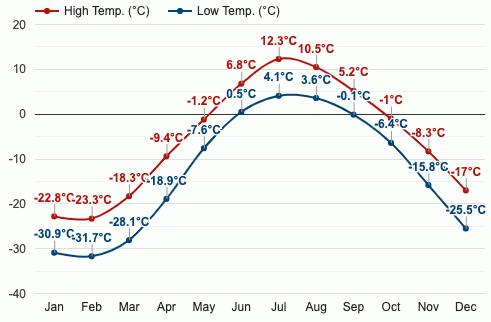
\includegraphics[scale=1.3]{thermo/diffusion/diffusionthermique/igloo.png}
    \caption{Variation de température à Whitehorse, Yukon, Canada.}
\end{figure}

\bigskip

\begin{center}
    \begin{minipage}{15cm}
        \textit{
        "The land itself was a desolation, lifeless, without movement, so lone and cold that the spirit of it was not even that of sadness. There was a hint in it of laughter, but of laughter more terrible than any sadness [...], a laughter cold as the frost and partaking of the grimness of infallibility. It was the Wild, the savage, frozen-hearted Northland Wild."}
        
        --- \quad \emph{White Fang}, Jack London
    \end{minipage}
\end{center}


\end{exercise}

\begin{solution}
\begin{questions}
    \question Voir le cours, on trouve l'équation de la chaleur
    \begin{align*}
        \pdv{T}{t} = \kappa \Delta T
    \end{align*}
    avec $\kappa = \frac{\lambda}{\mu c}$ la diffusivité thermique. Dans la couche de glace, les transferts thermiques se font par conduction. À l'intérieur de l'igloo il y a de l'air, les transferts thermiques se font par convection (bien plus rapidement que par conduction), on peut donc supposer que l'air à l'intérieur de l'igloo à une température homogène $T_i(t)$.
    
    \question (\textsf{Cas stationnaire}) Dans ce cas, on a $T = T(r)$, la température extérieure $T_0$ est constante ainsi que la température intérieure $T_i$. On a donc une équation de Laplace à résoudre : 
    \begin{align*}
        \Delta T = 0
    \end{align*}
    Avec comme condition aux limites :
    \begin{itemize}
        \item À l'extérieur de l'igloo, on prend une condition aux limites de type Dirichlet $T(R) = T_0$ (on pourrait aussi utiliser un modèle de flux conducto-convectif mais cela complexifierait le problème donc inutile de se lancer là-dedans si le sujet/l'examinateur ne vous y invite pas)
        \item À l'extérieur de l'igloo, on a une condition non pas sur la température (on ne connaît pas $T_i$ puisque c'est ce qu'on cherche) mais sur sa dérivée (condition de Neumann). Il faut dire que le flux total de chaleur sortant de l'intérieur de l'igloo $\phi$ est égal à la puissance thermique émise par la personne à l'intérieur $P$\footnote{Ordre de grandeur à connaître : la puissance thermique émise par un être humain lambda est de l'ordre de 100 W.}. Ce flux total est donc $\phi = \frac12 4\pi (R-h)^2 j(R-h) = P$, avec $j(R-h) = -\lambda \pdv{T}{r}(R-h)$.
    \end{itemize}
    On résout l'équation de Laplace (en utilisant la formule du laplacien en sphérique si on la connaît, en la retrouvant en faisant un bilan de chaleur sur une calotte hémisphérique infinitésimale sinon, cf cours) :
    \begin{align*}
         \frac1{r^2} \pdv{r}\qty(r^2\pdv{T}{r}) &= 0 \\
         \pdv{T}{r} &= -\frac{A}{r^2} \\
         T(r) &= B + \frac{A}{r}
    \end{align*}
    Et en utilisant que $T(R) = T_0$ et $\pdv{T}{r}(R-h) = -\frac{P}{2\pi \lambda (R-h)^2}$, on trouve $A = \frac{P}{2\pi \lambda}$ et $B = T_0 - \frac{P}{2\pi \lambda R}$, soit 
    \begin{align*}
        T(r) = T_0 + \frac{P}{2\pi \lambda}\qty(\frac1r-\frac1R)
    \end{align*}
    À ce stade, comme d'habitude, on vérifie que tout est bien homogène, on remarque que $T$ diminue lorsque $r$ augmente ce qui est toujours rassurant, et on peut même faire une petite application numérique pour trouver $T_i = T(R-h)$ en prenant des valeurs raisonnables de $P$, $R$ et $h$, $\lambda_{\text{glace}}$ étant fournie.
    
    \question (\textsf{Cas harmonique}) Cette fois-ci, la température extérieure n'est plus $T0$ mais $T_0 + \Delta T e^{i\omega t}$. Interprétation physique, cela correspond à une variation périodique de la température, le plus naturel a priori étant d'assimiler ceci à la variation des températures du rythme jour / nuit, on prendra donc pour les applications numériques $\omega = \frac{2\pi}{1\text{ jour}}$ et $\Delta T$ peut être obtenu en regardant l'écart moyen entre les deux courbes de la figure fournie.
    
    \question On a déjà déterminé la partie stationnaire de $T$, on étudie maintenant la partie oscillante. Cette fois-ci on doit écrire l'équation de diffusion dans toute sa généralité. Comme toujours dans ce genre de situations, on évite les fastidieux calculs du régime transitoire et on se place en régime permanent, on a donc $T(r, t) = \underline{T}(r) e^{i\omega T}$ avec $\underline{T} \in \mathbb{C}$. L'équation de la diffusion devient donc
    \begin{align*}
        i \omega \underline{T} = \kappa \Delta \underline{T} 
    \end{align*}
    Qui est donc une équation de Poisson
    \begin{align*}
        \Delta \underline{T} = i \frac{\underline{T}}{H^2}
    \end{align*}
    avec $H = \sqrt{\frac{\kappa}{\omega}}$ la taille caractéristique du problème. Puisque $\kappa$ la diffusivité thermique est une constante de diffusion comme son nom l'indique, $H$ est bien homogène à une longueur. Ouf !
    
    \question (\textsf{Résolution de l'équation}) Comme avant on écrit l'équation de Poisson :
    \begin{align*}
        \frac1{r^2} \pdv{r}\qty(r^2\pdv{T}{r}) &= i \frac{\underline{T}}{H^2}
    \end{align*}
    Qui a priori n'est pas triviale à résoudre. Malheur ! Heureusement, on peut faire confiance au colleur, qui nous a généreusement fourni un astucieux changement de variable (merci à lui). Suivant ses instruction les yeux fermés, on pose $f(r) = r \underline{T}(r)$ et on exprime l'équation en fonction de $f$ :
    \begin{align*}
        \pdv{r}\qty(r^2\pdv{r}\qty(\frac{f}{r})) &= i r\frac{f}{H^2} \\
        \pdv{r}\qty(r\pdv{f}{r} - f) &= i r\frac{f}{H^2} \\
        \pdv{f}{r} + r\pdv[2]{f}{r} - \pdv{f}{r} &= i r\frac{f}{H^2} \\
        \pdv[2]{f}{r} &= i \frac{f}{H^2}
    \end{align*}
    Qui est une équation d'oscillateur harmonique dont on connaît les solutions. Youpi ! \\
    Puisque $i = \qty(e^{i\frac{\pi}{4}})^2 = \qty(\frac{1+i}{\sqrt{2}})^2$, on peut réécrire l'équation
    \begin{align*}
        \pdv[2]{f}{r} &= \qty(\frac{1+i}{\sqrt{2}H})^2 f
    \end{align*}
    Dont les solutions sont évidentes : $f(r) = A\exp(\frac{1+i}{\sqrt{2}H}r) + B\exp(-\frac{1+i}{\sqrt{2}H}r)$, d'où l'on déduit $\underline{T}(r)$.
    
    \question (\textsf{Bilan}) La détermination exacte de $\underline{T}(r)$ ici est fastidieuse (il faudrait utiliser une forme astucieusement choisie de $f$ et appliquer rigoureusement les conditions aux limites en partie réelle et imaginaire). L'important est de voir que le module de la température varie proportionnellement à $e^{\frac{r}{H}}$, on peut donc dire grossièrement que l'igloo est ou pas sensible aux variations journalières de température selon que $h$ est plus grand ou plus petit que $H$. Une application numérique et un commentaure sont ici bienvenus.
    
    \question (\textsf{Bonus}) Il suffit comme précédemment d'utiliser la linéarité de l'équation pour superposer une seconde variation périodique de température $\Delta T '$ (pouvant être lu sur le graphe fourni) de fréquence $\omega' = \frac{2\pi}{1 \text{an}}$, et de reprendre le résultat précédent avec la nouvelle valeur $H'$.
\end{questions}

Pour conclure, un exercice qui commence par une question de cours standard (démonstration de l'équation de la chaleur) et se poursuit par une application très classique (résolution d'une équation de Laplace unidimensionnelle en géométrie sphérique). La situation est ensuite complexifiée par l'ajout d'une variation périodique, il suffit alors de suivre les raisonnements habituels en se laissant guider par les questions. Certaines questions sont volontairement imprécises, comme très souvent dans les exercices d'oraux, afin d'encourager la prise d'initiative et la discussion.

Il est de plus agrémenté d'un joli texte de Jack London, ce qui n'est pas sans contribuer à son intérêt !

\end{solution}
\begin{exercise}{Double vitrage}{1}{Spé}
{Diffusion thermique}{lelay, mines}

On souhaite poser une fenêtre en verre ($\lambda_v = 1.0$ W.m$^{-1}$.K$^{-1}$) d'un mètre carré dans une pièce devant être maintenue à 20 degrés Celsius. L'air extérieur à est 0 degrés Celsius.

\begin{questions}
    \questioncours Notion de résistance thermique
    \question Une vitre standard a comme épaisseur $e_v = 2$ mm. Quelle puissance faudra-t-il utiliser pour chauffer la pièce si on installe une vitre de ce type ? Cela vous parait-il raisonnable ?
    \question Quelle épaisseur doit faire la vitre si on veut ramener cette puissance à 400 W ? À 200 W ? Cela vous semble-t-il pratique ?
    \question On décide plutôt d'installer une fenêtre en double vitrage, composée de deux vitres épaisses de $e_v$ entre lesquelles il y a une épaisseur $e_a$ d'air ($\lambda_a = 0.02$ W.m$^{-1}$.K$^{-1}$). Quelle épaisseur $e_a$ d'air faut-il avoir pour n'avoir besoin que de 400 W pour chauffer la pièce ? Quelle est alors l'épaisseur totale de la fenêtre ?
    \question On souhaite réduire la puissance de chauffe à 200 W. Quelle épaisseur $e_a'$ d'air faut-il alors ? 
    \question En fait, on ne trouve pas de double vitrage avec une épaisseur $e_a'$ dans le commerce, seulement du triple vitrage constitué de trois plaques de verre entre lesquelles il y a deux couches d'air d'épaisseur $e_a'/2$ chacune. Pourquoi est-ce mieux ?
\end{questions}

\end{exercise}

\begin{exercise}{Isolation d'un salle de classe}{2}{Spé}
{Diffusion thermique}{lelay, mines}

On considère une salle de classe contenant $30$ élèves émettant chacun une puissance thermique de $60$ W. Cette salle est supposée calorifugée à l'exception d'un mur de la salle de surface $S_\text{m} = 30$ m$^2$, d'épaisseur $e_\text{m} = 20$ cm et de conductivité thermique $\lambda_\text{m} = 1.5$ W.m$^{-1}$.K$^{-1}$. Dans ce mur sont percées 5 fenêtres de conductivité thermique $\lambda_\text{f} = 1.0$ W.m$^{-1}$.K$^{-1}$ et d'épaisseur $e_\text{f} = 5$ mm, ayant chacune une surface $S_\text{f} = 1$ m$^2$. L'air extérieur est à $T_\text{e} = 10^\circ$C. On appelle $T_\text{i}$ la température à l'intérieur de la pièce.

\begin{questions}
    \questioncours Équation de la chaleur, notion de résistance thermique
    \question En supposant que la paroi extérieure des murs et des fenêtres soient à la température $T_\text{e}$, Quel est le flux de chaleur sortant par le mur ? Par les fenêtres ? Quelle est la principale cause des pertes thermiques ?
    \question En déduire la température d'équilibre $T_\text{i}$ de la pièce (pour laquelle la puissance thermique émise par les élèves compense celle des pertes thermiques).
    \question Quelle doit être la puissance des radiateurs de la salle pour que celle-ci soit maintenue à 20 degrés ?
    \uplevel{On considère maintenant que la paroi extérieure des fenêtres n'est pas à $T_\text{e}$ mais à $T_\text{s}$, et que le fenêtre échange à tout instant une puissance $P_\text{ech} = h S_\text{f} (T_\text{s}-T_\text{e})$ avec l'extérieur (modèle du flux conducto-convectif). On prendra $h = 20$ S.I.}
    \question D'où vient l'expression de $P_\text{ech}$ ? Quelle est l'unité de $h$ ?
    \question Qu'est-ce que cela change ? Avec ce modèle, $T_\text{i}$ sera-t-il a priori plus ou moins haut ?
    \question Calculer, avec ce modèle, $T_\text{i}$.
    \question Quelle doit être la puissance des radiateurs de la salle pour que celle-ci soit maintenue à 20 degrés ?
\end{questions}

\end{exercise}

\begin{exercise}{Isolation d'un bâtiment}{1}{Spé}
{Diffusion thermique}{lelay, mines}

On souhaite isoler un bâtiment d'habitation. On dispose pour cela de trois matériaux :
\begin{itemize}
    \item Le béton ($\lambda = 1.75$ W.m$^{-1}$.K$^{-1}$)
    \item Le plâtre ($\lambda = 1.50$ W.m$^{-1}$.K$^{-1}$)
    \item La laine de verre ($\lambda = 0.04$ W.m$^{-1}$.K$^{-1}$)
\end{itemize}

\begin{questions}
    \questioncours Flux d'énergie surfacique, loi de Fourier.
    \question Lequel de ces matériaux peut-être considéré comme un isolant thermique ?
    \question On décide de fabriquer le bâtiment avec des murs uniquement en béton (épaisseur 10 cm) recouvert du côté intérieur par une couche de plâtre (épaisseur 2 cm). Quelle puissance surfacique passe à travers des murs ainsi-conçu, pour une température intérieure de 20 degrés et extérieure de 5 degrés ?
    \question Que devient cette puissance si on ajoute 10 cm de laine de verre entre le béton et le plâtre ? Ce procédé est-il intéressant ?
    \question Donner la température moyenne du béton, de la laine de verre et du plâtre dans le dernier cas. 
\end{questions}

\end{exercise}

%\begin{exercise}{Ivre, il chute dans un ravin}{2}{Spé}
{Diffusion thermique}{bermu}

On souhaite isoler un bâtiment d'habitation. On dispose pour cela de trois matériaux :
\begin{itemize}
    \item Le béton ($\lambda = 1.75$ W.m$^{-1}$.K$^{-1}$)
    \item Le plâtre ($\lambda = 1.50$ W.m$^{-1}$.K$^{-1}$)
    \item La laine de verre ($\lambda = 0.04$ W.m$^{-1}$.K$^{-1}$)
\end{itemize}

\begin{questions}
    \questioncours Flux d'énergie surfacique, loi de Fourier.
    \question Lequel de ces matériaux peut-être considéré comme un isolant thermique ?
    \question On décide de fabriquer le bâtiment avec des murs uniquement en béton (épaisseur 10 cm) recouvert du côté intérieur par une couche de plâtre (épaisseur 2 cm). Quelle puissance surfacique passe à travers des murs ainsi-conçu, pour une température intérieure de 20 degrés et extérieure de 5 degrés ?
    \question Que devient cette puissance si on ajoute 10 cm de laine de verre entre le béton et le plâtre ? Ce procédé est-il intéressant ?
    \question Donner la température moyenne du béton, de la laine de verre et du plâtre dans le dernier cas. 
\end{questions}

\end{exercise}
 %pa fini

\section{Rayonnement du corps noir}

% Niveau :      PC
% Discipline :  Thermo
%Mots clés :    Rayonnement du corps noir

\begin{exercise}{Effet de serre}{2}{Spé}
{Thermodynamique, Rayonnement du corps noir}{bermu}

\begin{questions}
    \questioncours Qu'est-ce qu'un corps noir ? Rappeler les lois du déplacement de Wien et la loi de Stefan--Boltzmann.
    \question Quelle est la température effective $T_\text{ef}$ du soleil ? Évaluez le flux énergétique $I_0$ de ce dernier.
\uplevel{99,9\% du bilan énergétique de la Terre étant dû au rayonnement du Soleil, nous allons établir un modèle thermodynamique de la terre basé sur les échanges Soleil--Terre.}    
    \question Justifier que l'on puisse considérer la Terre comme un corps noir à condition de corriger le flux lumineux incident $I_0$ par $I_0 (1-A)$, $0<A<1$ étant l'albédo de la Terre. \\
    Tracer schématiquement le spectre en émission de la Terre.
    \question Quelle est la température d'équilibre $T_s$ en surface de la Terre ? Cette valeur vous paraît-elle cohérente ?
\uplevel{En fait, afin d'évaluer correctement la température de la terre il nous faut considérer le rôle majeur de l'atmosphère.}
    \question Rappeler ce qu'est l'effet de serre et le modéliser pour la Terre. \\
    On justifiera que l'atmosphère laisse passer intégralement les rayons du Soleil et absorbe les infrarouge.
    \question Calculer la température d'équilibre de la Terre pour $T\simeq 0$. Cela vous paraît-il  plus cohérent ?
    \question Qu'en est-il si on considère que l'atmosphère est un corps gris qui absorbe $\epsilon$ ($0<\epsilon<1$) dans l'IR et $\alpha$ ($0<\alpha<1$) dans le visible et que l'atmosphère et la surface de la Terre ont un albédo dans le visible $A_a$ et $A_s$ ? \\
    \'Etudier les cas limites.
    \question De quels facteurs environnementaux dépendent ces paramètres ?
\uplevel{L'effet de serre à un rôle majeur dans le réchauffement global ; si vous en doutez encore, le chimiste Svante Arhénius l'avait déjà prédit en 1895, mettez-vous à la page.}
    \question Faire un schéma des différentes boucles de rétroaction entraînant le réchauffement global.

%%% Mon bébé : c'est là où tu mets Fauve à l'honneur !

\end{questions}

\paragraph{Données :}
\begin{itemize}
    \item constante de Wien $b \simeq \dfrac{h c}{5 k_\textsc{b}} = 2,898\times 10^{-3}$ m$\cdot$K,
    \item constante de Stefan--Boltzmann $\sigma = 5,670\times 10^{-8}$ 
    $\mathrm{W\cdot m^{-2}\cdot K^{-4}}$,
    \item albédo de la Terre $A = 0,29$.
\end{itemize}
\end{exercise}

\section{Physique statistique}
% Niveau :      PC
% Discipline :  Electromagnétisme
%Mots clés :    Equations de Maxwell, Debye-Hückel


\begin{exercise}{Loi des gaz parfaits}{2}{Spé}
{Physique statistique,\'Electromagnétisme,Dipole électrostatique}{bermu}

On considère un gaz parfait de molécules de masse $m$ et de densité particulaire $n$ (en m$^{-3}$).

\begin{questions}
    \questioncours Loi de distribution des vitesses de Maxwell--Boltzmann. On notera $\ev{-}$ la moyenne associée.
    \question On considère une paroi, supposée immobile, de surface $\vec{S}$ et de normale $\vec{e}$ dans le gaz. Calculer quantité de mouvement $\delta\vec{p}_\text{paroi}$ communiquée par une particule de gaz de vitesse $\vec{v}$ sur cette paroi.
    \question En déduire la pression moyenne $P$ exercée par les particules du gaz $n$, $m$, $\vec{v}$ et $\vec{e}$ et $\ev{-}$.
    \question Retrouver la loi des gaz parfaits en calculant explicitement $\ev{-}$.
\end{questions}


\end{exercise}

\begin{solution}
\begin{questions}
    \questioncours $\mathbb{P}(v)\dd{v} \propto e^{-\frac{m v^2}{2 k_\textsc{b} T}}$
    \question Modèle simple : $\delta \vec{p}_\text{particule} = -\delta \vec{p}_\text{paroi}$.

    La paroi est immobile et collision élastique : $\delta \vec{p}_\text{paroi} = -2(m\vv\vdot\vec{e})\vec{e}$.
    \question Le bilan avec $\dd{N}$ particules qui collisionnent la paroi donne
    $\dd{\vec{p}} = \delta\vec{p}_\text{paroi}\dd{N}$, avec $\dd{N} = n \vec{S}\vdot\vv\dd{t}$.

    Modèle simplifié : 1/6 de particules dans chaque direction : $\dd{N} = n S v\dd{t}$, $\delta p_\text{paroi} = 2 m v$.

    Donc $\dv{p}{t} = P\times S =  2 m v \times \dfrac{1}{6} n v S = \dfrac{1}{3} n m v^2 S$.

    Ainsi $\ev{P} = \dfrac{1}{3} n m \ev{v^2}$ (sinon c'est sans l'hyopthèse $\ev{P} = 2 n m \ev{\qty(\vv\vdot\ve)^2}$).
    
    \question Or, $1/2 m\ev{v^2} = \#\text{ degré de libertés} \times \dfrac{1}{2} k_\textsc{b}T$.

    Donc $P = n k_\text{b}T$.
\end{questions}
\end{solution}

\begin{exercise}{Forces de Van der Waals}{2}{Spé}
{Physique statistique,\'Electromagnétisme,Dipole électrostatique}{bermu}

\begin{questions}
    \questioncours Distribution de Boltzmann.
    \question Quelle est l'expression du potentiel $V(\vr)$ et du champ $\vE(\vr)$ électriques
    \begin{parts}
        \part d'une charge ponctuelle $q$ ?
        \part d'un dipôle électrostatique permanent $\vec{p}$ ?
    \end{parts}
    \question Quelle est l'expression de l'énergie potentielle $\En_\text{p}$ exercée sur un dipôle par un champ électrique extérieur $\vE_\text{ext}$ ?
    \question Donner l'énergie potentielle $\En_\text{p}(r,\theta)$ exercée par une charge $q$ sur un dipôle permanent $\vec{p}$.
    \question Qu'en est-il si le dipôle $\vec{p}$ est induit ?
    \question $\norm{\vec{p}}$ et $\norm{\vec{r}}$ étant fixés, mais pas l'orientation du dipôle, qui fluctue dans le milieu, justifiez que le potentiel d'interaction effectif moyen $u_\text{eff}(r)$ puisse s'écrire :
    $$e^{-\beta u_\text{eff}(r)} = \dfrac{1}{2}\int_{\theta=0}^\pi e^{-\beta \En_\text{p}(r,\theta)} \sin\theta\dd{\theta}.$$
    \question Montrez à haute température (que cela veut-il dire ?) que $u_\text{eff}(r) \sim 1/r^4$, comme dans le cas du dipole induit.

    \plusloin

    \question Montrer que le potentiel d'interaction effectif entre deux dipôles(force de Keesom) est en $u_\text{eff}(r) \sim 1/r^6$. Interpréter.
\end{questions}


\end{exercise}

\begin{solution}
    \begin{questions}
        \question $\mathbb{P} \propto e^{-\cal{E}_\text{p}/k_\textsc{b}T}$
        \question \begin{align*}
            V_q(\vr) &= \dfrac{q}{4\pi\ep_0r} & \vec{E}_q(\vr) &= \dfrac{q\vec{e}_r}{4\pi\ep_0r^2} \\
            V_{\vec{p}}(\vr) &= \dfrac{\vec{p}\vdot\vec{e}_r}{4\pi\ep_0r^2} & \vec{E}_q(\vr) &= \dfrac{\qty(\vec{p}\vdot\vec{e}_r)\vec{e}_r - \vec{p}}{4\pi\ep_0r^3}
        \end{align*}
        \question \begin{align*}
           \vec{F}_{\vec{E}_\text{ext}/\vec{p}} &= -(\vec{p}\vdot\grad)\vec{E}_\text{ext} &
           \cal{E}_\text{p} &= -\vec{p}\vdot\vec{E}_\text{ext}
        \end{align*}
        \question $$\cal{E}_{\vec{p},q}(r,\theta) = \dfrac{q p \cos\theta}{4\pi\ep_0 r^2}$$
        \question Dans le cas du dipole induit $\vec{p} = \alpha \vec{E}$, donc on aurait :
        $$\cal{E}_{\vec{p},q}(r,\theta) = \dfrac{\alpha q^2}{(4\pi)^2\ep_0 r^4}$$
        \question Interprétation : on moyenne sur $\theta$ l'énergie d'intéraction.
        \question A haute température $T \gg T^\ast = \dfrac{q p}{4\pi\ep_0 r^2 k_\textsc{b}}$ :
        $$1-\beta u_\text{eff}(r) \simeq \dfrac{1}{2}\int_{\theta=0}^\pi \qty(1 - \beta k_\textsc{b} T^\ast \cos\theta + \beta^2 k_\textsc{b}^2 {T^\ast}^2 \cos^2\theta ) \sin\theta\dd{\theta} \simeq \dfrac{1}{6}\beta^2 k_\textsc{b}^2 {T^\ast}^2.$$
        Donc $$u_\text{eff} = \dfrac{q^2 p^2}{96\pi^2\ep_0^2 r^4 k_\textsc{b} T}$$
        On pourra donner que $\ev{\sin\theta\cos^2\theta} = \frac{2}{3}$.
        \question Dans le cas ou on a deux dipoles :
        $$\cal{E}_{\vec{p},q}(r,\theta) = \dfrac{(\vec{p}_1\vdot\vec{e}_r)(\vec{p}_1\vdot\vec{e}_r) - \vec{p}_1\vdot\vec{p}_2}{4\pi\ep_0 r^3}$$
        On aurait donc :
        $$e^{-\beta u_\text{eff}(r)} = \dfrac{1}{8\pi}\int_{\theta=0}^\pi e^{-\beta u(r)\cos\varphi\sin\theta_1\sin\theta_2} \sin\theta_1\dd{\theta_1}\sin\theta_2\dd{\theta_2}\dd{\varphi}.$$
        et donc $u_\text{eff} \sim 1/r^6$ : VdW !!
    \end{questions}
\end{solution}